\section{Rekonstrukcja powierzchni}
Wszystkie powyższe metody pozwalały na określenie chmury punktów danego obiektu. W celu wyeksportowania gotowego modelu, potrzebna jest również znajomość całej powierzchni danego przedmiotu. W tym pomocne okazują się różne metody rekonstrukcji powierzchni. Jest to kluczowy element działania algorytmu wirtualizacji rzeczywistych obiektów do postaci modeli 3D. Powstało wiele prac naukowych na temat różnych metod rekonstrukcji powierzchni, poniżej zostały omówione najważniejsze z nich.
\subsection{Trójwymiarowa triangulacja Delaunaya}
Triangulacja powierzchni metodą Delaunaya jest jedną z popularniejszych metod nakładania siatki na nieregularnie rozprowadzone punkty. Polega ona na połączeniu punktów w nieprzecinające się trójkąty, dzięki czemu możliwe jest nałożenie na nie koloru oraz utworzenie meshu na danym obiekcie. Triangulację Delaunaya można wykonać dla dowolnej N-wymiarowej płaszczyzny, w danym przykładzie zostanie opisana metoda dla trójwymiarowej chmury punktów \cite{cignoni1998dewall}. Schemat działania tej metody został opisany poniżej. 
\begin{enumerate}
    \item Tworzony jest czworościan zawierający wszystkie punkty ze zbioru.
    \item Tworzona jest lista czworościanów do usunięcia oraz czworościanów do pozostawienia.
    \item Dla każdego punktu sprawdzane jest czy leży on wewnątrz sfery opisanej na czworościanie do pozostawienia. Jeśli leży,to tworzone są 4 czworościany z wierzchołków starego oraz z nowego punktu.
    \Item Na końcu początkowy czworościan wewnątrz którego znajdowały się wszystkie punkty zostaje usunięty. Skasowane zostają również wszystkie czworościany mające z nim wspólny wierzchołek.
\end{enumerate}
Zaletą tej metody jest to, że jest ona inkrementacyjna. Punkty do triangulacji są dodawane po kolei,a co za tym idzie, nie ma potrzeby tworzenia nowej siatki po dodaniu pojedynczego punktu. Wystarczy jedynie wykonać jedną fazę algorytmu i dopisać utworzone wierzchołki czworościanów do listy.
Modyfikacją tej metody jest triangulacja DeWall zaproponowana przez włoskich naukowców w 1997 roku \cite{cignoni1998dewall}. Jej nazwa pochodzi od Delaunay i ściana (ang. \textit{Wall}). Pojęcie ściany oznacza w tym wypadku rekurencyjne dzielenie zbioru punktów na dwa podobne do siebie obszary, następnie równoległe utworzenie dwóch niezależnych od siebie triangulacji Delaunaya. Dzięki podzieleniu zbioru punktów na niezależne od siebie obszary, możliwe staje się wykorzystanie wielowątkowości procesora do obliczeń równoległych. To znacząco przyspiesza pracę algorytmu.
\subsection{Algorytm maszerujących sześcianów}
Algorytm maszerujących sześcianów jest metodą typu dziel i podbijaj zaproponowaną w 1987 roku przez amerykańskich naukowców w Nowym Yorku \cite{lorensen1987marching}. W przeciwieństwie do triangulacji Delaunaya, punkty na które ma zostać nałożona siatka meshu muszą być w regularnych odstępach od siebie. W związku z tym, chcąc wykorzystać tę metodę trzeba dokonać interpolacji punktów, w celu przejścia z nieregularnych przestrzeni pomiędzy elementami do równomiernie leżących punktów. Ze względu na schemat działania algorytmu, jest on niezwykle szybki, ponieważ pozwala on na uniknięcie części obliczeń. Algorytm dzieli przestrzeń na regularne sześciany, a następnie sprawdza przecięcia punktów ze ścianami sześcianu. Przy regularnej siatce punktów istnieje $2^8$ takich przecięć, ponieważ sześcian ma 8 krawędzi, na każdej z nich może leżeć punkt lub nie. Po uwzględnieniu symetrii obrotowej sześcianu liczbę kombinacji można zredukować do zaledwie 15. Zostały one przedstawione na rysunku ~\ref{fig:marchingCubesCut}.
\begin{figure}[H]
  \centering
  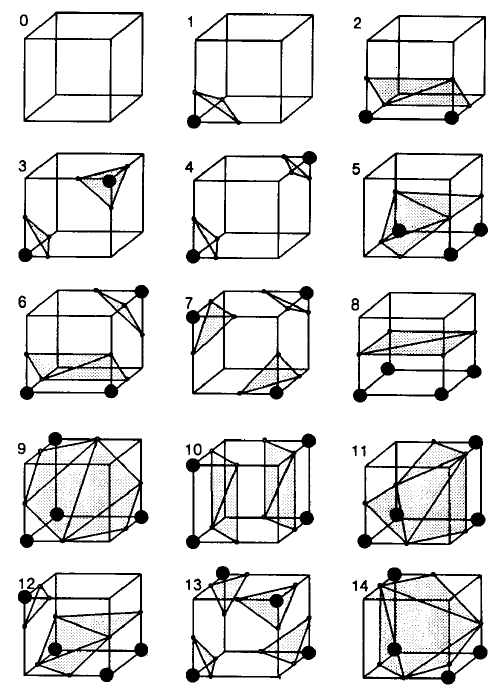
\includegraphics[scale=0.5]{przeciecia.PNG}
  \caption{Możliwe przecięcia sześcianu przez punkty \cite{lorensen1987marching}}   
  \label{fig:marchingCubesCut}
\end{figure}
Przecięcia punktów z sześcianami tworzą trójkąty, które później zostaną dodane do triangulacji. Należy zwrócić uwagę na to, że gęstość meshu na obiekcie poddanym triangulacji bezpośrednio zależy od długości boku sześcianu. Im jest on mniejszy, tym więcej będzie przecięć punktów z krawędziami, a co za tym idzie, więcej utworzonych trójkątów triangulacyjnych. Występują odmiany tej metody wprowadzające zmienną długość boku danego sześcianu \cite{shu1995adaptive}. Adaptacyjna metoda maszerujących sześcianów bada krzywiznę powierzchni wewnątrz sześcianów za pomocą wyznaczania wektorów normalnych utworzonych dla danych trójkątów. Jeśli wektory odchylone są w podobną stronę, oznacza to, że powierzchnia jest dostatecznie gładka. W przeciwnym wypadku sześcian dzielony jest na kolejne cztery sześciany i algorytm jest powtarzany do momentu uzyskania odpowiedniej krzywizny powierzchni. Dzięki wykorzystaniu tej metody tworzona jest dokładniejsza triangulacja powierzchni względem początkowego algorytmu. Ponadto dzięki wykorzystaniu adaptacyjnej metody algorytm jest szybszy niż ten który by miał ustalona długość boku. Porównanie algorytmu maszerujących sześcianów oraz jej adaptacyjnej odmiany dla różnych ilości punktów znajduje się w tabeli ~\ref{tab:amcvsmc}.

\begin{table}[H]
\begin{center}
\caption{\label{tab:amcvsmc}Porównanie algorytmu MS oraz adaptacyjnych MS dla 7.4\cdot $10^6$ oraz 2.8\cdot $10^6$ punktów \cite{shu1995adaptive}.}
\begin{tabular}{ |c| c|c|c|c| }
 \hline
 {\small Metoda} & {\small MS}&{ \small AMS} & {\small MS}&{ \small AMS}\\ 
  \hline
     {\small Liczba punktów } & {\small  7.4\cdot $10^6$ } & {\small  7.4\cdot $10^6$ } & {\small  2.8\cdot $10^6$ } & {\small  2.8\cdot $10^6$ }   \\  
  \hline
     {\small Czas trwania } & {\small 331 s} & {\small 230 s}& {\small 164 s} & {\small 81 s}    \\  
  \hline
   {\small  Ilość trójkątów } & {\small 718964 } & {\small 299292 }& {\small 393606 } & {\small 102868 }  \\  
  \hline
\end{tabular}
\end{center}
\end{table}



\subsection{Ball pivoting algorithm}

Algorytm toczącej się kuli jest metodą służącą do rekonstrukcji powierzchni na podstawie chmury punktów. Został on zaproponowany przez Fausto Bernardini i pozostałych w 1999 roku \cite{bernardini1999ball}. BPA został stworzony by szybko i dokładnie odwzorowywać kształt powierzchni. Schemat postępowania programu, opiera się o kulę, która toczy się po powierzchni punktów. Z początku, wybierany jest pierwszy trójkąt triangulacyjny. Trzy punkty utworzą pierwszy trójkąt triangulacyjny, jeśli kula styka się tylko i wyłącznie z nimi. Gdy tocząc się ,kula natrafi na dodatkowy punkt, to zostaje on połączony z bokiem wcześniejszego trójkąta. Cały proces powtarza się do momentu, gdy kula pokona całą powierzchnię. Pomimo przejścia kuli przez całą powierzchnię, nie oznacza to, że ze wszystkich punktów zostanie utworzony mesh. Warto nadmienić, że głównym parametrem wpływającym na czas trwania algorytmu jest promień kuli. W większości przypadków, ustala się go na podstawie średniej odległości punktów od siebie. Jeśli promień będzie niedostatecznie duży, to kula może "wypaść" przez punkty, więc nie zostaną one połączone. Powstają wtedy dziury, które negatywnie wpływają na ostateczny wygląd meshu. Można je później załatać wykorzystując algorytmy interpolacji liniowej lub ponownie uruchomić algorytm BPA, tym razem z większym promienień i powtórzyć cały proces jeszcze raz. W efekcie czego większość dziur zostanie załatana. Wpłynie to jednak na znaczne zwiększenie czasu trwania algorytmu. Wizualizacja zasady działania algorytmu została przedstawiona na rysunku ~\ref{fig:bpaZasada}

\begin{figure}[H]
  \centering
  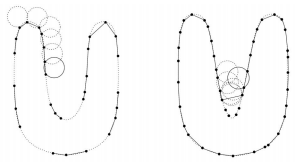
\includegraphics[scale=0.8]{bpa_zasada.PNG}
  \caption{Zasada działania algorytmu BPA \cite{bernardini1999ball}}   
  \label{fig:bpaZasada}
\end{figure}
Główną zaletą tego algorytmu jest fakt, że jego złożoność obliczeniowa zależy liniowo od ilości punktów w zbiorze. Jeśli dodany zostanie dodatkowy punkt, to kula musi się przez niego przetoczyć kilka razy. Jednak cała struktura pozostałych punktów pozostaje niezmienna. Ten aspekt algorytmu stanowi największą odmianę względem triangulacją Delaunay'a. W triangulacji Delaunay'a, po dodaniu dodatkowego punktu cała struktura triangulacji może się zmienić. Ważną zaletą algorytmu jest możliwość regulacji promienia kuli R, im promień jest mniejszy, tym algorytm zajmie więcej czasu, ponieważ zetknie się z mniejszą ilością punktów podczas toczenia. Zatem eksperymentując z długością promienia, można otrzymać zadowalająco dobre rezultaty w krótszym czasie. 


